\documentclass[aspectratio=169]{beamer}

\usepackage[utf8]{inputenc}

\usepackage{color}
\usepackage{listings}
\usepackage{tikz}
\usepackage{hyperref}

\usetheme{Rochester}
\usecolortheme{beaver}

\lstloadlanguages{C++}
    \lstset{%
        language={C++},
        basicstyle=\ttfamily,
        keywordstyle=\color{blue},
        showstringspaces=false,
        escapechar={§},
        escapeinside=||
    }

\newif\iftransitions
% \transitionstrue


\newif\iffast
% \fasttrue

\title{Type Punning Done Right}
%\subtitle{Lua for C++ Programmers}
\author{Andreas Weis}
\institute{BMW AG}
\date{Meeting C++, November 11, 2017}
%\titlegraphic{
\includegraphics[height=.25\textheight]{resources/cppcon.png}}


\begin{document}

\frame{\titlepage}

\begin{frame}[fragile]
  \frametitle{About me}

  \begin{itemize}
    \setlength\itemsep{1.5em}

    \item \href{https://stackoverflow.com/users/577603/comicsansms}{
\includegraphics[height=.05\textheight]{resources/so-icon.png}} \href{https://github.com/ComicSansMS}{
\includegraphics[height=.05\textheight]{resources/github-icon.png}} 
\includegraphics[height=.05\textheight]{resources/slack-icon.png} Known as ComicSansMS on most sites

    \item \href{https://twitter.com/DerGhulbus/}{
\includegraphics[height=.05\textheight]{resources/twitter-icon.png} @DerGhulbus on Twitter}

    \item 
\includegraphics[height=.05\textheight]{resources/meetup-icon.png} Co-organizer of the \href{https://www.meetup.com/MUCplusplus/}{Munich C++ User Group}

    \item Currently working as a Software Architect for BMW 
\includegraphics[height=.1\textheight]{resources/bmw_group.jpg}

  \end{itemize}
\end{frame}


\begin{frame}[fragile]
  \frametitle{What is type punning?}

  Accessing data through a pointer of unrelated type.

  The act of type punning itself does not change the underlying data.

  It controls the \emph{operations} applied to that data.
\end{frame}


\begin{frame}[fragile]
  \frametitle{Types control operations}
  \setlength{\tabcolsep}{12pt}
  \begin{columns}
    \column{0.4\linewidth}
 
    \begin{lstlisting}
template<typename T>
void increment_impl(T& n) {
    ++n;
}
    \end{lstlisting}
    \pause
    \begin{lstlisting}
void increment(float& f) {
    increment_impl(f);
}

void increment(int& i) {
    increment_impl(i);
}
    \end{lstlisting}
    \pause
    \column{0.5\linewidth}
    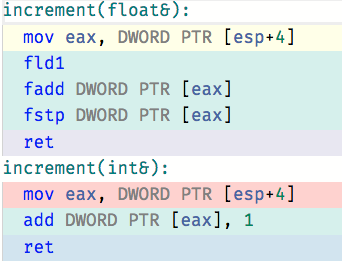
\includegraphics[height=.8\textheight]{resources/increment_float_int.png}
  \end{columns}
\end{frame}


\begin{frame}[fragile]
  \frametitle{Aliasing}

  Aliasing is when the same thing is accessed through different names.

  \begin{lstlisting}
void foo(int* a, int* b) {
  *a = 1;
  *b = 2;
}

int x = 42;
foo(&x, &x);
  \end{lstlisting}

  Aliasing forces the compiler to respect a corner case that is unlikely to ever occur in practice.

  Fortran does not allow aliasing in this case and might thus be able to generate faster code here.

  C99 introduced the \texttt{restrict} keyword to indicate alias-free pointers.
\end{frame}


\begin{frame}
  \frametitle{Strict Aliasing in C and C++}

  Type-based aliasing: If two pointers have different types, they must not alias.

  Effectively makes na"ive type punning illegal.
\end{frame}

\begin{frame}[fragile]
  \frametitle{Type punning done right}

  \begin{lstlisting}
float next_ulp(float f)
{
    static_assert(sizeof(float) == sizeof(uint32_t));
    uint32_t tmp;
    memcpy(&tmp, &f, sizeof(float));
    ++tmp;
    memcpy(&f, &tmp, sizeof(float));
    return f;
}
  \end{lstlisting}
\end{frame}


\begin{frame}[fragile]
  \frametitle{a}

  \begin{lstlisting}
float next_ulp(float f) {
    (*(int*)(&f))++;
    return f;
}
  \end{lstlisting}
\end{frame}



\begin{frame}
  \frametitle{Thanks for your attention.}
\end{frame}


\end{document}
